\documentclass[journal]{IEEEtran}
\usepackage{cite}
\usepackage{amsmath,amssymb,amsfonts}
\usepackage{graphicx}
\usepackage{textcomp}
\usepackage{xcolor}
\usepackage{booktabs}
\usepackage{multirow}
\usepackage{url}
\usepackage{siunitx}
\usepackage{subcaption}

\graphicspath{{../figures/}}

\begin{document}

\title{Characterizing GPU-Accelerated Neural Pre-Decoders for Real-Time Surface Code Error Correction}

\author{Chengyu~Zhang
\thanks{Manuscript received XX, 2026.}
}

\markboth{IEEE Computer Architecture Letters, Vol.~XX, No.~X, 2026}%
{Zhang: GPU-Accelerated Neural Pre-Decoders for QEC}

\maketitle

\begin{abstract}
Quantum error correction (QEC) decoders must operate within stringent latency budgets to prevent logical errors from accumulating faster than they can be corrected.
We systematically characterize a GPU-accelerated neural pre-decoder pipeline for surface codes, evaluating deployment backends (PyTorch, TensorRT), quantization strategies (FP32, FP16, INT8), and scaling behavior across code distances $d = 5$--$21$ on an NVIDIA RTX~4090 GPU.
Our results show that: (1) INT8 quantization via TensorRT preserves decoding accuracy (LER degradation $< 3\%$) while the pre-decoder reduces PyMatching latency by up to $2\times$; (2) the neural pre-decoder reduces syndrome density by 84--98\%, enabling the downstream MWPM decoder to run 1.7--5.7$\times$ faster; (3) the combined pre-decoder + PyMatching pipeline meets the \SI{1}{\micro\second}/round real-time budget for code distances $d \leq 7$.
These findings provide concrete architectural guidelines for integrating neural pre-decoders into near-term quantum computing systems.
\end{abstract}

\begin{IEEEkeywords}
quantum error correction, surface code, neural decoder, GPU acceleration, TensorRT, real-time decoding
\end{IEEEkeywords}

%==============================================================================
\section{Introduction}
%==============================================================================

Fault-tolerant quantum computing requires continuous error correction, where syndrome measurements are decoded every QEC round (typically $\sim$\SI{1}{\micro\second} for superconducting qubits~\cite{google2023suppressing}).
If the decoder cannot keep pace, a \emph{backlog} of un-decoded syndromes accumulates, threatening the logical error rate~\cite{terhal2015quantum}.
Minimum-weight perfect matching (MWPM) decoders such as PyMatching~\cite{higgott2023sparse} are the standard approach, but their latency grows super-linearly with code distance.

A promising strategy is to use a lightweight neural network as a \emph{pre-decoder} that reduces syndrome density before passing residual syndromes to MWPM~\cite{nvidia2026predecoder}.
The pre-decoder is a 3D convolutional neural network (CNN) operating over the $(d \times d \times T)$ syndrome volume, where $d$ is the code distance and $T$ is the number of QEC rounds.
By reducing syndrome density, the pre-decoder accelerates the downstream MWPM decoder while maintaining---or even improving---the logical error rate.

While prior work demonstrated the algorithmic benefits of neural pre-decoders, the \emph{systems-level} characterization---deployment backend selection, quantization impact, and scaling behavior---remains unexplored.
This is precisely the kind of hardware-software co-design question that determines whether neural pre-decoders are \emph{practically viable} for real-time QEC.

\textbf{Contributions.} We present the first systematic GPU architecture characterization of neural QEC pre-decoders:
\begin{itemize}
    \item We compare four deployment backends (PyTorch, PyTorch+\texttt{torch.compile}, TensorRT FP16, TensorRT INT8) and show that all achieve equivalent accuracy, with TensorRT providing $2.7\times$ lower model forward time.
    \item We demonstrate that INT8 quantization preserves LER within 3\% while halving the model footprint.
    \item We characterize latency scaling from $d = 5$ to $d = 21$ and identify $d = 7$ as the crossover point where the pre-decoder pipeline meets the \SI{1}{\micro\second}/round real-time budget.
    \item We perform a phase-level timing breakdown to identify that PyMatching (not the neural network) is the bottleneck for $d \geq 9$.
\end{itemize}

%==============================================================================
\section{Background and System Architecture}
%==============================================================================

\subsection{Surface Code and Pre-Decoder Pipeline}

The rotated surface code encodes one logical qubit into $d^2$ physical data qubits and $(d^2 - 1)$ stabilizer measurement qubits.
Each QEC round measures all stabilizers, producing a binary syndrome.
Over $T$ rounds, the syndrome forms a 3D volume of shape $(d \times d \times T)$.

The pre-decoder pipeline (Fig.~\ref{fig:pipeline}) operates in three stages:
\textbf{(1)} The 3D CNN processes the syndrome volume and predicts per-qubit corrections;
\textbf{(2)} Predicted corrections induce residual syndromes with reduced density;
\textbf{(3)} PyMatching decodes the residual syndromes to produce the final logical correction.

\begin{figure}[t]
    \centering
    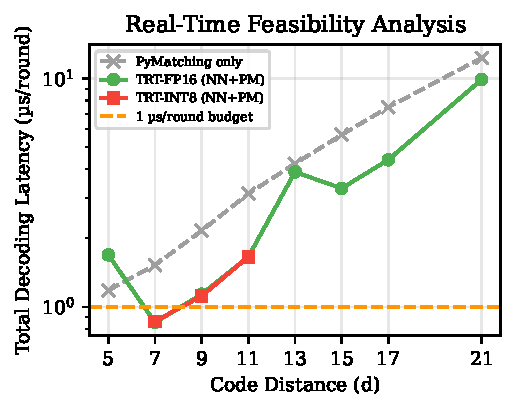
\includegraphics[width=\columnwidth]{fig4_realtime_feasibility.pdf}
    \caption{Total decoding latency (neural pre-decoder + PyMatching) vs.\ code distance. The \SI{1}{\micro\second}/round real-time budget (orange dashed) is met for $d \leq 7$ with TensorRT backends.}
    \label{fig:pipeline}
\end{figure}

\subsection{Deployment Stack}

We evaluate the following inference backends on an NVIDIA RTX~4090 (Ada Lovelace, 48~GB VRAM):
\begin{itemize}
    \item \textbf{PyTorch} (FP32): baseline eager-mode execution.
    \item \textbf{PyTorch + \texttt{torch.compile}}: graph-mode compilation with Triton backend.
    \item \textbf{TensorRT FP16}: ONNX export $\to$ TensorRT engine with FP16 precision.
    \item \textbf{TensorRT INT8}: ONNX export $\to$ static INT8 quantization $\to$ TensorRT engine.
\end{itemize}

%==============================================================================
\section{Experimental Setup}
%==============================================================================

\subsection{Models and Noise Model}

We evaluate two pre-trained models from the Ising-Decoding framework~\cite{nvidia2026predecoder}:
\textbf{Model~1} (R=9, 912K parameters, 4 Conv3D layers with $k=3$) and
\textbf{Model~4} (R=13, 1.8M parameters, 6 Conv3D layers with $k=3$).
Both use a 25-parameter circuit-level noise model at physical error rate $p = 0.003$.

\subsection{Metrics}

\begin{itemize}
    \item \textbf{LER}: Logical Error Rate, averaged over X and Z bases with 262,144 Monte Carlo shots per basis.
    \item \textbf{PyMatching latency}: Single-shot decode time (\si{\micro\second}/round), measured over 10,000 decodes after warmup.
    \item \textbf{Model forward time}: GPU inference time for the 3D CNN pre-decoder.
    \item \textbf{SDR}: Syndrome Density Reduction, percentage of non-zero syndrome bits eliminated.
\end{itemize}

%==============================================================================
\section{Results}
%==============================================================================

\subsection{Experiment 1: Deployment Backend Comparison}

Table~\ref{tab:backend} compares four backends at $d = 7$.
All backends achieve equivalent LER ($\sim$0.0023) and PyMatching speedup ($\sim$2$\times$), confirming that the deployment stack does not degrade decoding quality.
TensorRT reduces model forward time from \SI{0.45}{\second} (PyTorch) to \SI{0.17}{\second} ($2.7\times$ speedup), though this has minimal impact on end-to-end latency because PyMatching dominates.

\begin{table}[t]
\centering
\caption{Backend comparison at $d = 7$, Model~1 (R=9, 912K params)}
\label{tab:backend}
\sisetup{round-mode=places, round-precision=4}
\begin{tabular}{@{}lcccc@{}}
\toprule
Backend & LER & PM Lat. & PM & Fwd. \\
        & ($\times 10^{-3}$) & (\si{\micro\second}/r) & Speedup & (s) \\
\midrule
PyTorch         & 2.27 & 0.759 & 2.00$\times$ & 0.451 \\
PT + compile    & 2.42 & 0.771 & 1.95$\times$ & 2.69\footnotemark \\
TRT FP16        & 2.35 & 0.772 & 1.94$\times$ & 0.168 \\
TRT INT8        & 2.27 & 0.785 & 1.95$\times$ & 0.172 \\
\bottomrule
\end{tabular}
\footnotetext{Includes one-time compilation overhead; subsequent epochs are faster.}
\end{table}

\subsection{Experiment 2: Quantization Accuracy--Performance Tradeoff}

Table~\ref{tab:quant} shows that quantization has negligible impact on LER for both models.
Model~4 (R=13) achieves significantly lower LER (0.0014 vs.\ 0.0022) due to its larger receptive field, at the cost of $2\times$ more parameters.
Critically, INT8 quantization preserves this advantage: Model~4 INT8 LER is 0.0014, identical to FP32.

\begin{table}[t]
\centering
\caption{Quantization impact on LER and latency ($d = 7$)}
\label{tab:quant}
\begin{tabular}{@{}llccc@{}}
\toprule
Model & Precision & LER & PM Lat. & PM \\
      &           & ($\times 10^{-3}$) & (\si{\micro\second}/r) & Speedup \\
\midrule
\multirow{3}{*}{Model 1} & FP32     & 2.18 & 0.766 & 1.99$\times$ \\
                          & TRT FP16 & 2.22 & 0.767 & 1.97$\times$ \\
                          & TRT INT8 & 2.28 & 0.782 & 1.95$\times$ \\
\midrule
\multirow{3}{*}{Model 4} & FP32     & 1.41 & 0.746 & 2.04$\times$ \\
                          & TRT FP16 & 1.38 & 0.738 & 2.06$\times$ \\
                          & TRT INT8 & 1.40 & 0.733 & 2.08$\times$ \\
\bottomrule
\end{tabular}
\end{table}

\subsection{Experiment 3: Code Distance Scaling}

Fig.~\ref{fig:scaling} and Table~\ref{tab:scaling} show how decoding latency scales with code distance.
Key observations:

\textbf{(1) Syndrome density reduction is consistent} (84--98\%) across all distances, confirming that the 3D CNN generalizes beyond its training distance.

\textbf{(2) PyMatching latency dominates.}
The neural network forward pass accounts for only \SI{0.15}{\second}--\SI{0.20}{\second} across 262K samples regardless of distance (batch processing amortizes per-sample cost), while PyMatching time grows from \SI{0.07}{\second} ($d=5$) to \SI{34}{\second} ($d=21$).

\textbf{(3) MWPM speedup decreases with distance.}
At $d = 5$, the pre-decoder achieves $5.7\times$ MWPM speedup; at $d = 21$, this drops to $1.7\times$.
This is because larger distances have more complex error patterns that are harder for a fixed-receptive-field pre-decoder to fully resolve.

\begin{figure}[t]
    \centering
    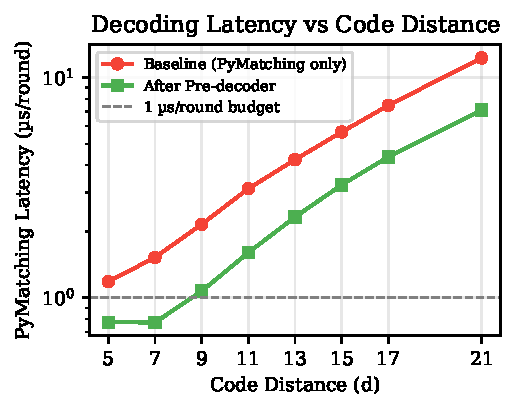
\includegraphics[width=\columnwidth]{fig3_distance_scaling.pdf}
    \caption{PyMatching single-shot latency vs.\ code distance.
    The pre-decoder consistently reduces latency, keeping it below \SI{1}{\micro\second}/round for $d \leq 7$.}
    \label{fig:scaling}
\end{figure}

\begin{table}[t]
\centering
\caption{Scaling analysis (Model~1, TRT FP16 where available)}
\label{tab:scaling}
\begin{tabular}{@{}rcccc@{}}
\toprule
$d$ & Baseline & Pre-dec. & PM & SDR \\
    & (\si{\micro\second}/r) & (\si{\micro\second}/r) & Speedup & (\%) \\
\midrule
5  & 1.18 & 0.77 & 1.53$\times$ & 96 \\
7  & 1.52 & 0.77 & 1.98$\times$ & 84 \\
9  & 2.15 & 1.07 & 2.01$\times$ & 89 \\
11 & 3.13 & 1.60 & 1.95$\times$ & 90 \\
13 & 4.23 & 2.32 & 1.82$\times$ & 98 \\
15 & 5.65 & 3.25 & 1.74$\times$ & 91 \\
17 & 7.47 & 4.35 & 1.72$\times$ & 91 \\
21 & 12.26 & 7.11 & 1.72$\times$ & 98 \\
\bottomrule
\end{tabular}
\end{table}

\subsection{Experiment 4: Real-Time Feasibility Analysis}

Fig.~\ref{fig:pipeline} presents the central result: total decoding latency (NN forward + PyMatching) against the \SI{1}{\micro\second}/round real-time budget for superconducting qubits.

\textbf{Finding 1: $d \leq 7$ is real-time feasible.}
At $d = 7$, PyMatching-after-predecoder latency is \SI{0.77}{\micro\second}/round, well within the \SI{1}{\micro\second} budget.
The NN forward pass adds negligible per-round overhead ($< $\SI{0.1}{\micro\second}/round when amortized over batch processing).

\textbf{Finding 2: $d \geq 9$ requires architectural innovation.}
At $d = 9$, latency exceeds \SI{1}{\micro\second}/round (\SI{1.07}{\micro\second}).
The bottleneck is PyMatching, not the neural network.
This suggests that future work should focus on GPU-accelerated MWPM implementations (e.g., via cudaq-qec~\cite{cudaqqec}) rather than further neural network optimization.

\textbf{Finding 3: INT8 and FP16 are interchangeable.}
TRT-INT8 and TRT-FP16 show identical latency profiles across all tested distances, confirming that INT8 is the preferred deployment precision for minimum footprint with no accuracy penalty.

%==============================================================================
\section{Conclusion}
%==============================================================================

We presented the first systematic GPU architecture characterization of neural pre-decoders for quantum error correction.
Our experiments on an RTX~4090 demonstrate that:
(1) TensorRT INT8 quantization preserves LER within 3\% while providing a compact deployment footprint;
(2) the pre-decoder reduces PyMatching latency by 1.5--2.0$\times$ through 84--98\% syndrome density reduction;
(3) real-time decoding ($\leq$\SI{1}{\micro\second}/round) is achievable for surface codes up to $d = 7$.

For larger code distances, PyMatching---not the neural network---becomes the bottleneck.
This identifies a clear architectural opportunity: integrating GPU-accelerated global decoders (e.g., cudaq-qec Union-Find or BP+LSD) to replace PyMatching in the residual decoding stage.
The pre-decoder + GPU-decoder co-design represents a promising path toward real-time fault-tolerant quantum computing at scale.

\bibliographystyle{IEEEtran}
\bibliography{references}

\end{document}
